\section{{Results and Discussion}}

We follow a condition through the pipeline in order; the first three stages are measured against the human annotation without any language model, the fourth with the official metric.

\subsection{Chunking separates conditions from the answers they qualify}
\label{sec:chunking}

With 150-word chunks, the gold of \sepCond\% of conditional questions no longer fits in a single chunk, against \sepUncond\% of unconditional ones; a conditional question needs \goldChunksCond{} gold chunks on average against \goldChunksUncond. For \condOnly\% of conditional questions at least one condition sits in a chunk holding no other evidence the answer needs. Larger chunks reduce separation without removing it: \sepCondThreeHundred\% are still split at 300 words (mean \chunkWordsThreeHundred{} words) and \sepCondHundred\% at 100 (mean \chunkWordsHundred). Structure, not size, is what helps: section-aware chunks (a new chunk at every top-level heading, mean \chunkWordsSection{} words) split \sepCondSection\% and isolate a condition in \condOnlySection\% of conditional questions, while size-matched fixed 70-word chunks split \sepCondSeventy\% and isolate one in \condOnlySeventy\%. On gov.uk pages conditions are typically list items under a lead-in sentence or paragraphs below a rule, so the structure that states a condition is the structure a word budget cuts.

\subsection{Retrieval finds conditions as often as answers, except those chunked apart}
\label{sec:retrieval}

At $k=8$ the hybrid retriever returns \recAnsEight\% of answer chunks and \recCondEight\% of condition chunks of conditional questions, and the two curves stay together at every depth (Figure~2). The exception is the chunk that holds a condition and nothing else: only \recCondOnlyEight\% are retrieved at $k=8$, and they trail the other curves until $k=50$. The full gold reaches the generator for \recAllGoldEight\% of conditional questions, and when every answer chunk has been retrieved a condition chunk is still missing in \recLostGivenAnsEight\% of cases: the configuration that yields a confident answer without its caveat. Section-aware chunks cover less text at the same $k$, so condition recall falls to \recCondEightSection\% and complete-gold recall to \recAllGoldEightSection\%.

\textbf{Context-preserving retrieval designs do not consistently improve condition coverage.} Held to the top 8's word budget (\blWordsTop{} words on average), sentence windows, parent--child sections, hierarchical page-then-chunk retrieval and condition-expanded queries give a condition coverage (the share of gold condition elements of conditional questions in the context) of \blRecallSentwin\%, \blRecallParent\%, \blRecallHier\% and \blRecallQexp\%, against \blRecallTop\% for the top 8, and the whole gold for \blCompleteSentwin\%, \blCompleteParent\%, \blCompleteHier\% and \blCompleteQexp\% of questions, against \blCompleteTop\%. End to end, on the answerable questions of the hosted subsample, the four designs change F1 with conditions on conditional questions against the top 8 by \blCondMin{} to \blCondMax{} points across the two local generators; \blCondNSig{} of these \blNRuns{} differences, and \blUncondNSig{} on unconditional questions, are distinguishable from zero.

\begin{figure}[!htbp]\centering
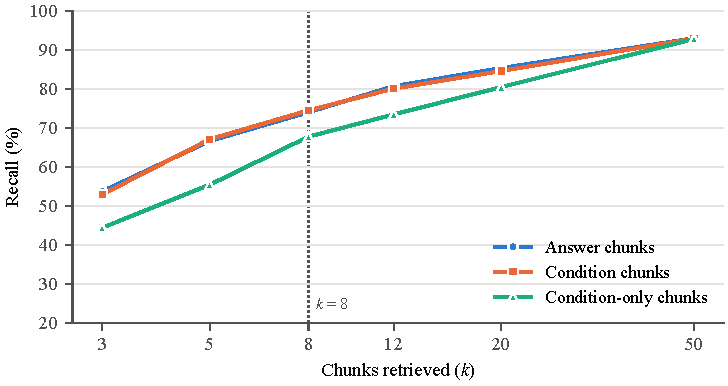
\includegraphics[width=0.56\textwidth]{recall.pdf}
\vspace{3pt}\\
\textbf{Figure 2.} Recall of gold chunks against retrieval depth for the \nEvalCond{} conditional evaluation questions (hybrid retrieval over \nChunks{} chunks). Condition-only chunks hold a condition and no other gold evidence.
\end{figure}

\subsection{The evaluated operators do not distinguish conditions}
\label{sec:operators}

The model-free operators choose chunks before any answer is generated, so their effect on conditions is measured directly (Figure~3, left). Reranking the top 8 down to 3 removes \rrCondDrop\% of the retrieved condition chunks and \rrAnsDrop\% of the answer chunks. The contradiction filter changes the context of \nliChanged\% of conditional questions, although every passage comes from one consistent body of guidance, and removes \nliCondDrop\% of condition chunks and \nliAnsDrop\% of answer chunks; the ConflictRAG-style resolver changes \crsChanged\% of contexts and removes \crsCondDrop\% and \crsAnsDrop\%. None of them targets conditions, and none protects them. To an NLI model an exception contradicts the rule it qualifies: for one evaluation question the filter kept ``You'll get a `Certificate of Destruction' to prove that the vehicle has been destroyed'' and dropped, with contradiction probability 1.00, the gold condition ``You will not get a certificate of destruction if the ATF decides to repair and sell your vehicle''. On RAMDocs, where removing documents is the purpose, the same operators do not single out misinformation either (Figure~3, right): reranking keeps \ramRrMisinfo\% of misinformation documents and \ramRrCorrect\% of correct ones, since a document with one entity swapped is exactly as relevant as the original, and the filter keeps \ramNliMisinfo\% and \ramNliCorrect\%.

\begin{figure}[!htbp]\centering
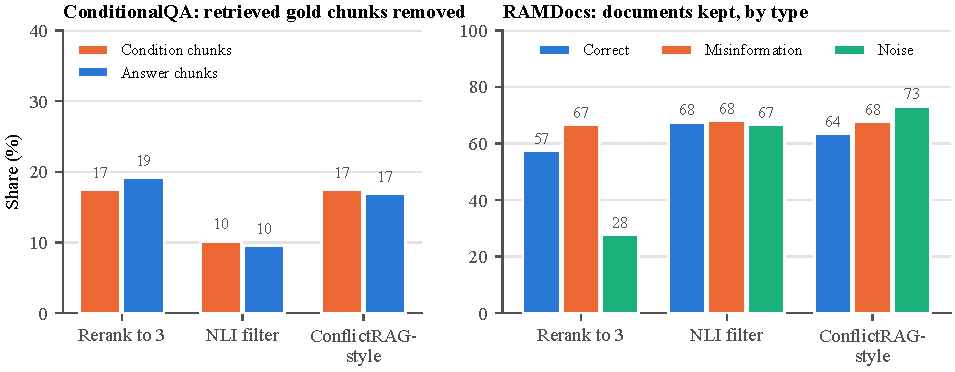
\includegraphics[width=0.78\textwidth]{operators.pdf}
\vspace{3pt}\\
\textbf{Figure 3.} Left: share of the gold condition and answer chunks retrieved in the top 8 that each operator removes (\nOpCond{} conditional evaluation questions with a retrieved condition chunk). Right: share of RAMDocs documents each operator keeps, by type (\nRamQ{} questions).
\end{figure}

\subsection{Generation and the choice of prompt}
\label{sec:generation}

Already on the tuning set, with exactly the gold chunks in context, the generators mark only \tunRecallQwen\% (Qwen2.5-7B), \tunRecallLlama\% (Llama-3.1-8B) and \tunRecallBig\% (Qwen3.8-27B) of the gold conditions as conditions, and F1 with conditions on these questions is \tunFcCondQwen, \tunFcCondLlama{} and \tunFcCondBig{}, against 56.6 for the benchmark's human annotators \cite{sun2022conditionalqa}. The metric rewards silence: a stated condition scores zero whenever the gold has none, as for most questions. For Qwen2.5-7B, a wording that discourages conditions (v2) cut the unconditional answers naming one to \tunAnyCondUncondVTwo\% and raised F1 with conditions on unconditional questions to \tunFcUncondVTwo, while it fell to \tunFcCondVTwo{} on conditional ones. We froze the wording that states the benchmark's own definition of a condition (v4: \tunFcCondQwen{} and \tunFcUncondVFour), not the one with the best overall score, because a generator that rarely states conditions cannot lose one, and every comparison of evidence policies would then show no effect by construction.

Is the generation deficit then a property of this prompt? Table~3 answers the hosted subsample with the gold chunks under five condition-aware strategies besides the frozen one (analysis v). No strategy removes the deficit. Across six prompts and three generators, the share of gold conditions stated as conditions ranges from \prMinRecall\% to \prMaxRecall\%, and is at most \prMaxRecallLocal\% for the local models. Against the frozen prompt, \prNSigGain{} of the \prNRuns{} variant runs raise F1 with conditions on conditional questions by an amount distinguishable from zero (largest change \prMaxGain{} points) and \prNSigLoss{} lower it; the largest gain, answer--condition pairing with Nemotron-3-Ultra, still states only \prRecallNemoPairing\% of the gold conditions and changes F1 with conditions on unconditional questions by \prVsUncondNemoPairing. The strategies that state more conditions attach them to more unconditional answers too: direct extraction raises the condition recall of Llama-3.1-8B from \prRecallLlamaVFour\% to \prRecallLlamaExtract\% and of Nemotron-3-Ultra from \prRecallNemoVFour\% to \prRecallNemoExtract\%, but changes F1 with conditions on unconditional questions by \prVsUncondLlamaExtract{} and \prVsUncondNemoExtract, and \prNSigLossUncond{} of the \prNRuns{} variant runs are significantly worse there. Chain-of-condition reasoning, whose identify-and-verify steps target exactly this failure, gives condition recall of \prRecallQwenCoc\%, \prRecallLlamaCoc\% and \prRecallNemoCoc\%, against \prRecallQwenVFour\%, \prRecallLlamaVFour\% and \prRecallNemoVFour\% with the frozen prompt. Removing the condition-only chunks lowers F1 with conditions under \prCTwoPos{} of the \prCTwoN{} prompt--generator combinations, so the chunking cost does not depend on the prompt either. The deficit is not an artefact of one wording, though it remains a finding about the strategies we evaluated.

% Generated by study/report.py. Do not edit by hand.
\begin{table}[!htbp]\centering
\textbf{Table 3.} The generation deficit under six prompts, with the gold chunks in context (hosted subsample: 150 conditional, 100 unconditional questions). Rec.: share of gold conditions stated as conditions (\%); on U: share of unconditional answers that name any condition (\%); F1c: F1 with conditions on conditional / unconditional questions (\%). The first row is the frozen prompt; the other five were added in revision (exploratory) and share its lines, worked examples and output format.\\\vspace{5pt}
{\fontsize{9}{11}\selectfont
\setlength{\tabcolsep}{3.5pt}
\begin{tabular}{L{3.3cm}P{0.8cm}P{0.8cm}P{1.75cm}P{0.8cm}P{0.8cm}P{1.75cm}P{0.8cm}P{0.8cm}P{1.75cm}}
\toprule
 & \multicolumn{3}{c}{\textbf{Qwen2.5-7B}} & \multicolumn{3}{c}{\textbf{Llama-3.1-8B}} & \multicolumn{3}{c}{\textbf{Nemotron-3-Ultra}} \\
\textbf{Prompting strategy} & Rec. & on U & F1c C / U & Rec. & on U & F1c C / U & Rec. & on U & F1c C / U \\
\midrule
frozen: the benchmark's definition & 21.6 & 36.0 & 10.0 / 30.7 & 18.1 & 26.0 & 15.2 / 59.2 & 32.1 & 17.0 & 19.2 / 58.3 \\
direct condition extraction & 15.1 & 46.0 & 11.2 / 21.0 & 28.2 & 45.0 & 16.0 / 42.1 & 42.5 & 38.0 & 19.6 / 47.1 \\
answer--condition pairing & 23.8 & 36.0 & 13.2 / 33.9 & 16.4 & 25.0 & 13.6 / 50.2 & 38.6 & 22.0 & 24.5 / 53.6 \\
chain-of-condition reasoning & 11.2 & 22.0 & 5.1 / 26.8 & 20.8 & 47.0 & 11.3 / 36.0 & 30.7 & 15.0 & 18.4 / 58.3 \\
applicability check per line & 15.6 & 28.0 & 10.4 / 32.8 & 11.2 & 28.0 & 9.1 / 55.6 & 36.7 & 25.0 & 18.9 / 54.4 \\
evidence first, roles labelled & 14.8 & 39.0 & 7.7 / 18.4 & 20.0 & 46.0 & 12.9 / 38.2 & 35.9 & 28.0 & 19.7 / 48.2 \\
\bottomrule
\end{tabular}
}
\end{table}


\subsection{End to end: where the conditions are lost}
\label{sec:endtoend}

Table~4 lists every system on the evaluation set and Table~5 the pre-registered tests; the two local generators agree on every confirmatory comparison but the last. \textbf{The metric measures condition use:} deleting the condition elements from the gold chunks lowers F1 with conditions by \cOneQwenPt{} for Qwen2.5-7B and \cOneLlamaPt{} for Llama-3.1-8B (C1). \textbf{Chunking costs conditions:} on the \nCondOnlyEval{} conditional questions with a condition-only gold chunk, removing those chunks from the gold context costs \cTwoQwenPt{} and \cTwoLlamaPt{} (C2), although everything else the answer needs is present. \textbf{Retrieval costs a little; dilution costs more:} at an equal budget of eight chunks, the gold chunks filled up with distractors beat the top 8 by \cThreeQwenPt{} and \cThreeLlamaPt{} (C3), so most of the distance between the gold chunks and the top 8 (\fcGoldQwen{} against \fcTopQwen{} for Qwen2.5-7B, \fcGoldLlama{} against \fcTopLlama{} for Llama-3.1-8B) is what retrieval adds, not what it misses.

\textbf{The operators change nothing measurable at this scale.} Reranking, the contradiction filter and the ConflictRAG-style resolver each leave F1 with conditions within about a point of the top 8 (C4--C6), although they remove \rrCondDrop\%, \nliCondDrop\% and \crsCondDrop\% of the retrieved condition chunks: these generators state so few conditions that there is little to lose, citing \noticedTopQwen\% and \noticedTopLlama\% of the condition lines they are shown in the top 8. \textbf{Context completion does not help:} under the clean threshold protocol it changes F1 with conditions against the top 8 by \clCSevenQwenPt{} and \clCSevenLlamaPt{} (C7; Holm-adjusted $p$ of \clCSevenHolmQwen{} and \clCSevenHolmLlama), and on unconditional questions it meets the non-inferiority margin of 2 points for Qwen2.5-7B (lower bound \clCEightLowQwen) but not for Llama-3.1-8B (\clCEightLowLlama); the pre-registered protocol gives \cSevenQwenPt{} and \cSevenLlamaPt{} (C7$^{\mathrm{p}}$) and the same non-inferiority verdicts. Of the exploratory policies only listwise selection, in which the reader itself chooses the chunks, gains for both generators (\eSevenQwen{} and \eSevenLlama), distinguishably from zero only for Llama-3.1-8B. \textbf{Closed-book answering is a sobering baseline:} without evidence, Qwen2.5-7B scores \fcClosedUncondQwen{} on unconditional questions, far above the \fcTopUncondQwen{} it reaches with the top 8, which tempts it to attach a condition to \anyCondTopUncondQwen\% of answers that need none. On the \nOppositeQwen{} conditional questions whose gold contains both ``yes'' and ``no'', the gold chunks beat the top 8 by \eSixQwen{} and \eSixLlama{}, the same direction as on all conditional questions.

% Generated by study/report.py. Do not edit by hand.
\begin{center}
\textbf{Table 3.} End-to-end results on the evaluation set: F1 with conditions (\%) on conditional (C) and unconditional (U) questions, and the share of gold condition elements in the context that the generator cites anywhere (noticed, \%).\\\vspace{5pt}
{\fontsize{10}{12}\selectfont
\begin{tabular}{L{4.6cm}P{1.35cm}P{1.35cm}P{1.35cm}P{1.35cm}P{1.35cm}P{1.35cm}}
\toprule
 & \multicolumn{3}{c}{\textbf{Qwen2.5-7B}} & \multicolumn{3}{c}{\textbf{Llama-3.1-8B}} \\
\textbf{System} & F1c (C) & noticed & F1c (U) & F1c (C) & noticed & F1c (U) \\
\midrule
\multicolumn{7}{l}{\emph{Oracle ladder}}\\
\texttt{closed-book} & -- & -- & -- & -- & -- & -- \\
\texttt{gold} & -- & -- & -- & -- & -- & -- \\
\texttt{gold\,$-$\,cond.\ elements} & -- & -- & -- & -- & -- & -- \\
\texttt{gold\,$-$\,cond.-only chunks} & -- & -- & -- & -- & -- & -- \\
\texttt{gold\,+\,distractors} & -- & -- & -- & -- & -- & -- \\
\midrule
\multicolumn{7}{l}{\emph{Retrieval}}\\
\texttt{top-3} & -- & -- & -- & -- & -- & -- \\
\texttt{top-8} & -- & -- & -- & -- & -- & -- \\
\midrule
\multicolumn{7}{l}{\emph{Evidence-reducing operators}}\\
\texttt{rerank-3} & -- & -- & -- & -- & -- & -- \\
\texttt{NLI filter} & -- & -- & -- & -- & -- & -- \\
\texttt{ConflictRAG-style} & -- & -- & -- & -- & -- & -- \\
\texttt{listwise selection} & -- & -- & -- & -- & -- & -- \\
\midrule
\multicolumn{7}{l}{\emph{Context completion}}\\
\texttt{adjacent} & -- & -- & -- & -- & -- & -- \\
\texttt{page} & -- & -- & -- & -- & -- & -- \\
\texttt{completion (untrained)} & -- & -- & -- & -- & -- & -- \\
\texttt{completion} (ours) & -- & -- & -- & -- & -- & -- \\
\bottomrule
\end{tabular}
}
\end{center}


% Generated by study/report.py. Do not edit by hand.
\begin{table}[!htbp]\centering
\textbf{Table 5.} The pre-registered confirmatory family: paired difference in F1 with conditions (points), 95\% BCa interval over pages, and Holm-adjusted page-level sign-flip $p$. C: conditional questions; C$^\dagger$: those with a condition-only gold chunk; U: unconditional. C8 asks whether the lower bound exceeds $-2$ points.\\\vspace{5pt}
{\fontsize{10}{12}\selectfont
\begin{tabular}{L{0.6cm}L{3.95cm}P{0.85cm}P{2.65cm}P{1.05cm}P{2.65cm}P{1.05cm}}
\toprule
 & & & \multicolumn{2}{c}{\textbf{Qwen2.5-7B}} & \multicolumn{2}{c}{\textbf{Llama-3.1-8B}} \\
\textbf{ID} & \textbf{Comparison} & \textbf{Pop.} & diff.\ [95\% CI] & $p_{\mathrm{Holm}}$ & diff.\ [95\% CI] & $p_{\mathrm{Holm}}$ \\
\midrule
C1 & gold vs.\ cond.\ elements deleted & C & +7.1 [+5.4, +9.1] & $<$0.001 & +9.9 [+7.6, +12.3] & $<$0.001 \\
C2 & gold vs.\ cond.-only chunks removed & C$^\dagger$ & +5.2 [+2.6, +8.3] & 0.004 & +5.7 [+2.6, +9.4] & 0.005 \\
C3 & gold + distractors vs.\ top-8 & C & +1.2 [+0.3, +2.0] & 0.025 & +1.1 [+0.5, +1.9] & 0.013 \\
C4 & rerank-3 vs.\ top-8 & C & $-$0.0 [$-$1.6, +1.4] & 1.000 & +1.0 [$-$0.5, +2.6] & 0.690 \\
C5 & NLI filter vs.\ top-8 & C & $-$0.3 [$-$1.3, +0.6] & 1.000 & +0.6 [$-$0.5, +1.6] & 0.690 \\
C6 & ConflictRAG-style vs.\ top-8 & C & $-$0.4 [$-$1.4, +0.4] & 1.000 & $-$0.4 [$-$1.5, +0.7] & 0.690 \\
C7 & completion vs.\ top-8 & C & $-$0.0 [$-$1.2, +1.2] & 1.000 & +1.3 [$-$0.1, +2.7] & 0.390 \\
C8 & completion vs.\ top-8 (non-inferiority) & U & +3.7 [+0.8, +7.3] & yes & $-$2.5 [$-$6.1, +1.2] & no \\
\bottomrule
\end{tabular}
}
\end{table}


\subsection{Inside the generation loss}
\label{sec:diagnostics}

We measure outputs, not comprehension: a gold condition in the context can be cited at all, cited as a condition, and cited as a condition only when the scenario leaves it open. The output format separates the first two (Table~6), and the dominant failure is the first. With the gold chunks in context, Qwen2.5-7B leaves \decGoldNotCitedQwen\% of the gold conditions uncited, Llama-3.1-8B \decGoldNotCitedLlama\% and even Nemotron-3-Ultra \decGoldNotCitedNemo\%; citing a condition only as evidence accounts for less (\decGoldEvOnlyOss\% to \decGoldEvOnlyLlama\%). Matching explains little of this. Crediting a stated element that restates a missed gold condition (token F1 at least 0.5) adds \auditRestateMin{} to \auditRestateMax{} points of recall across the five generators, and a loose criterion (a third of words shared) at most \auditLooseMax{}; crediting a stated element that the NLI model judges equivalent (mutual entailment) adds at most \semMutualMax{} points, and one that merely entails or is entailed by the gold condition at most \semEitherMax, leaving every recall at or below \semEitherRecallMax\%. Stated conditions are often wrong: \decGoldSpurQwen\% of those Qwen2.5-7B states are not gold conditions, many of them lines stating the answer itself.

% Generated by study/report.py. Do not edit by hand.
\begin{table}[!htbp]\centering
\textbf{Table 7.} What happens to the gold conditions in the context (conditional questions: \nEvalCond{} for the local generators, 150 for the hosted ones): the share stated as a condition (Cond.), cited only as evidence (Ev.) or not cited at all (None), with gold and with top-8 context; and, with gold context, the share of stated conditions that are not gold conditions (Spur.) and, of those, the share that are lines stating the answer (Ans.); answer F1 ignoring conditions (F1) and exact match with conditions (EM$_c$) on the conditional questions; and the share of unconditional answers that name any condition (FC). All values in \%.\\\vspace{5pt}
{\fontsize{10}{12}\selectfont\setlength{\tabcolsep}{3.8pt}
\begin{tabular}{L{2.7cm}P{0.84cm}P{0.84cm}P{0.84cm}P{0.84cm}P{0.84cm}P{0.84cm}P{0.84cm}P{0.84cm}P{0.84cm}P{0.84cm}P{0.84cm}}
\toprule
 & \multicolumn{3}{c}{\textbf{gold}} & \multicolumn{3}{c}{\textbf{top-8}} & \multicolumn{5}{c}{\textbf{gold}} \\
\textbf{Generator} & Cond. & Ev. & None & Cond. & Ev. & None & Spur. & Ans. & F1 & EM$_c$ & FC \\
\midrule
Qwen2.5-7B & 21.0 & 15.6 & 63.5 & 17.9 & 13.4 & 68.7 & 77.4 & 25.8 & 41.8 & 8.2 & 39.0 \\
Llama-3.1-8B & 18.2 & 19.1 & 62.7 & 9.7 & 13.6 & 76.7 & 61.9 & 48.5 & 50.2 & 12.5 & 26.5 \\
gpt-oss-20b & 21.1 & 12.9 & 66.0 & 16.4 & 12.4 & 71.2 & 57.9 & 54.7 & 49.7 & 14.5 & 32.0 \\
Gemma-4-31B & 27.9 & 15.3 & 56.7 & 23.2 & 18.0 & 58.8 & 44.3 & 58.0 & 56.7 & 22.1 & 13.0 \\
Nemotron-3-Ultra & 32.1 & 17.5 & 50.4 & 22.8 & 20.4 & 56.8 & 44.8 & 52.6 & 47.8 & 15.9 & 17.0 \\
\bottomrule
\end{tabular}
}
\end{table}


\textbf{A dedicated condition check} recovers many conditions but cannot tell when none applies. With gold context it raises condition recall from \revVerGoldCondQwenRecallBase\% to \revVerGoldCondQwenRecall\% for Qwen2.5-7B and from \revVerGoldCondLlamaRecallBase\% to \revVerGoldCondLlamaRecall\% for Llama-3.1-8B, and F1 with conditions on conditional questions by \revVerGoldCondQwenPt{} and \revVerGoldCondLlamaPt; but it attaches a condition to \revVerGoldUncondQwenAny\% and \revVerGoldUncondLlamaAny\% of unconditional answers (from \revVerGoldUncondQwenAnyBase\% and \revVerGoldUncondLlamaAnyBase\%), often a line stating the answer itself, and F1 with conditions there changes by \revVerGoldUncondQwenPt{} and \revVerGoldUncondLlamaPt. Nemotron-3-Ultra and Gemma-4-31B behave alike (recall \revVerGoldCondNemoRecallBase\% to \revVerGoldCondNemoRecall\% and \revVerGoldCondGemmaRecallBase\% to \revVerGoldCondGemmaRecall\%; unconditional F1 with conditions \revVerGoldUncondNemoPt{} and \revVerGoldUncondGemmaPt). Prompted to look, a generator cites many more of the conditions in its context; but extracting a condition does not show that it can judge whether the scenario leaves it open, and the gain on conditional questions is paid for several times over on unconditional ones.

\textbf{Section-aware chunks end to end} keep more conditions with their answers but are retrieved less completely, and the two nearly cancel: with the top 8 the share of gold conditions in the context falls from \revSecTopCondQwenCtxBase\% to \revSecTopCondQwenCtx\%, and F1 with conditions on conditional questions changes by \revSecTopCondQwenPt{} and \revSecTopCondLlamaPt; re-cutting only the gold chunks changes it by \revSecGoldCondQwenPt{} and \revSecGoldCondLlamaPt. With the top 8, Qwen2.5-7B leaves \unansTopQwen\% of unanswerable questions unanswered and Llama-3.1-8B \unansTopLlama\%, and no evidence policy moves either by more than a few points.

\subsection{Why context completion does not help}
\label{sec:completion}

The completion scorer is weak at its task. Over the candidate chunks of the evaluation questions, \qPosPairs{} of which hold a gold condition and \qNegPairs{} do not, it ranks a condition chunk above a non-condition chunk with probability \qAucTrained, below the \qAucZero{} of the untrained reranker it was meant to improve on. Under the clean protocol, with fold thresholds from \clThMin{} to \clThMax, its AUC is \clAuc{} and it adds \clAdded{} chunks per question, only \clPrec\% of which hold a condition (pre-registered threshold: \qAddedTrained{} chunks, \qPrecTrained\%). Neither the candidate pool nor the threshold is the bottleneck: \ceilMissedInPool\% of the condition chunks the top five miss lie on the pages completion searches, and a threshold chosen on the evaluation questions themselves raises the scorer's F1 only to \sweepBestTrained{} (untrained: \sweepBestZero). Condition chunks are rare among the candidates, share their page, topic and vocabulary with the chunks around them, and are conditions only relative to a scenario that leaves them open, which a pairwise relevance scorer sees only indirectly.

A better scorer would not change the conclusion much. \texttt{completion (oracle)} adds exactly the missed condition chunks, raising the share of gold conditions in the context from \revOracleCondQwenCtxBase\% to \revOracleCondQwenCtx\%; yet the condition recall of Qwen2.5-7B rises only from \revOracleCondQwenRecallBase\% to \revOracleCondQwenRecall\% and that of Llama-3.1-8B from \revOracleCondLlamaRecallBase\% to \revOracleCondLlamaRecall\%, and F1 with conditions changes against the top 8 by \revOracleCondQwen{} and \revOracleCondLlama{}. For the two larger generators recall does not rise (\revOracleCondNemoRecallBase\% to \revOracleCondNemoRecall\% for Nemotron-3-Ultra, \revOracleCondGemmaRecallBase\% to \revOracleCondGemmaRecall\% for Gemma-4-31B). While the generator fails to state most conditions it is given, completion's ceiling is set by generation, not by the scorer. Nor does what the scorer learns transfer: on the transfer corpus it does not rank the \oodPosNatural{} refinement pairs above the \oodNegNatural{} pairs not in conflict (AUC \oodAucNatural, 95\% CI \oodAucNaturalLow{} to \oodAucNaturalHigh; probe pairs \oodAucProbes). It has learned where conditions sit on a ConditionalQA page, not what makes one passage qualify another. This is a negative result for our implementation, not for qualifier-aware retrieval in general.

\subsection{Larger generators}
\label{sec:hosted}

Table~7 repeats four systems with three larger generators on the stratified subsample of \nHostedQ{} questions. These exploratory comparisons test direction only; with 150 conditional questions (\hCondOnlyN{} with a condition-only gold chunk) the intervals are wide, and the evidence is the paired differences with their intervals, not the point estimates. The models differ in architecture, training, serving and reasoning settings as well as size, so no ordering of them by parameter count is supported.

The direction of every main effect holds, and the losses before generation do not shrink. Removing the condition-only chunks costs gpt-oss-20b \hCTwoOss, Gemma-4-31B \hCTwoGemma{} and Nemotron-3-Ultra \hCTwoNemo, and on the same questions Qwen2.5-7B \hCTwoQwenSamePt{} and Llama-3.1-8B \hCTwoLlamaSamePt; replacing the gold chunks by the top 8 costs \hEOneOssPt, \hEOneGemmaPt{} and \hEOneNemoPt, against \hEOneQwenSamePt{} and \hEOneLlamaSamePt. Generation still shows the largest observed deficit: with exactly the gold chunks in context, the three models state \hRecallOss\%, \hRecallGemma\% and \hRecallNemo\% of the gold conditions as conditions (F1 with conditions \hGoldOss, \hGoldGemma{} and \hGoldNemo), so even the 550B-parameter model fails to state about two thirds of them as conditions. Completion, run with the pre-registered threshold for these models, helps none of them: against the top 8 it changes F1 with conditions by \hCSevenOssPt, \hCSevenGemmaPt{} and \hCSevenNemoPt{} (only Gemma's change is distinguishable from zero). Groq served \hServedGroqOss{} of the \hServedTotalOss{} gpt-oss-20b calls and NVIDIA the rest; on the questions Groq answered, the two providers' F1 with conditions differs by \provDiff.

% Generated by study/report.py. Do not edit by hand.
\begin{center}
\textbf{Table 5.} Larger hosted generators on the stratified subsample (150 conditional, 100 unconditional questions): F1 with conditions (\%) on conditional (C) and unconditional (U) questions, and conditions noticed (N, \%) as in Table 3.\\\vspace{5pt}
{\fontsize{10}{12}\selectfont
\begin{tabular}{L{3.6cm}P{0.85cm}P{0.85cm}P{0.85cm}P{0.85cm}P{0.85cm}P{0.85cm}P{0.85cm}P{0.85cm}P{0.85cm}}
\toprule
 & \multicolumn{3}{c}{\textbf{gpt-oss-20b}} & \multicolumn{3}{c}{\textbf{Gemma-4-31B}} & \multicolumn{3}{c}{\textbf{Nemotron-3-Ultra}} \\
\textbf{System} & C & N & U & C & N & U & C & N & U \\
\midrule
\texttt{gold} & 17.2 & 34.0 & 50.4 & 25.2 & 43.3 & 62.8 & 19.2 & 49.6 & 58.3 \\
\texttt{gold\,$-$\,cond.-only chunks} & 13.7 & 37.3 & -- & 21.6 & 44.1 & -- & 14.9 & 51.7 & -- \\
\texttt{top-8} & 12.6 & 28.8 & 44.9 & 16.8 & 41.2 & 55.8 & 14.1 & 43.2 & 55.6 \\
\texttt{completion} (ours) & 13.2 & 34.5 & 42.7 & 14.3 & 38.7 & 55.3 & 12.0 & 47.1 & 53.5 \\
\bottomrule
\end{tabular}
}
\end{center}


\subsection{The same operators where discarding is right}
\label{sec:ramdocs}

On RAMDocs (Table~8) the room for an operator is large: discarding exactly the misinformation and noise raises strict accuracy on the questions with misinformation from \ramFullMiQwen\% to \ramOracleMiQwen\% for Qwen2.5-7B and from \ramFullMiLlama\% to \ramOracleMiLlama\% for Llama-3.1-8B. None of the operators captures any of it. On those questions, reranking to three documents changes strict accuracy by \ramRerankEffQwenPt{} and \ramRerankEffLlamaPt, the contradiction filter by \ramNliEffQwenPt{} and \ramNliEffLlamaPt, and the resolver by \ramCrsEffQwenPt{} and \ramCrsEffLlamaPt; three of these six intervals lie wholly below zero, none above it. Over all questions the filter (\ramNliEffAllQwenPt{} and \ramNliEffAllLlamaPt) and the resolver (\ramCrsEffAllQwenPt{} and \ramCrsEffAllLlamaPt) are significantly worse than keeping every document ($p<0.001$ for all four). Listwise selection answers fewer misinformation questions wrongly but loses correct answers as fast (\ramSelectEffAllQwenPt{} and \ramSelectEffAllLlamaPt{} overall).

Four capabilities are at stake here and should be kept apart: detecting that two passages contradict each other, judging which source is credible, establishing which statement is true, and recognising that one passage limits where another applies. A valid exception contradicts the rule it qualifies, and two documents that agree can both be false, so success at the first says little about the others. The operators we evaluated decide what to remove by relevance, apparent contradiction or, for the resolver, surface credibility cues; on these data they deliver neither factual correctness on RAMDocs nor condition preservation on ConditionalQA, although the two datasets' absolute scores are not comparable.

% Generated by study/report.py. Do not edit by hand.
\begin{center}
\textbf{Table 6.} The same operators on RAMDocs, where discarding is correct: strict accuracy (\%) on all questions and on those with misinformation (MI), and the share of MI answers that state a wrong answer.\\\vspace{5pt}
{\fontsize{10}{12}\selectfont
\begin{tabular}{L{4.0cm}P{1.45cm}P{1.45cm}P{1.45cm}P{1.45cm}P{1.45cm}P{1.45cm}}
\toprule
 & \multicolumn{3}{c}{\textbf{Qwen2.5-7B}} & \multicolumn{3}{c}{\textbf{Llama-3.1-8B}} \\
\textbf{System} & all & MI & wrong (MI) & all & MI & wrong (MI) \\
\midrule
\texttt{full context} & -- & -- & -- & -- & -- & -- \\
\texttt{oracle discard} & -- & -- & -- & -- & -- & -- \\
\texttt{rerank-3} & -- & -- & -- & -- & -- & -- \\
\texttt{NLI filter} & -- & -- & -- & -- & -- & -- \\
\texttt{ConflictRAG-style} & -- & -- & -- & -- & -- & -- \\
\texttt{relevance grading} & -- & -- & -- & -- & -- & -- \\
\texttt{listwise selection} & -- & -- & -- & -- & -- & -- \\
\bottomrule
\end{tabular}
}
\end{center}

